\documentclass[a0paper,25pt,portrait,blockverticalspace=20mm, colspace=20mm]{tikzposter}

\usepackage{etex}
%\usepackage{authblk}
\usepackage{amsmath,amsthm,mathrsfs,amssymb,amsfonts,dsfont,nicefrac,stmaryrd,yhmath}
\usepackage{mathtools,cancel}
\mathtoolsset{showonlyrefs=true}
\usepackage{multicol}
\usepackage{csquotes}
\usepackage{bold-extra,moresize}
\usepackage{layout}
\usepackage{tikz,pgfplots}
\pgfplotsset{compat=newest}
\usepackage{pgfmath,pgffor}
\usetikzlibrary{plotmarks}
\usepackage{pgfplotstable}
\usepackage{pgfpages}
\usepackage{tikz-3dplot}

\usetikzlibrary{datavisualization, patterns}
\usetikzlibrary{arrows,positioning,shapes,trees,mindmap,shadows} 
\usepgfplotslibrary{fillbetween}
\usepgfplotslibrary{colormaps}
\usepgfplotslibrary{colorbrewer}
\usepgfplotslibrary{external}
\usepgfplotslibrary{groupplots}
\usetikzlibrary{decorations.markings,intersections,calc}
\usetikzlibrary{decorations.pathreplacing}
\usetikzlibrary{fit}
%%%%%%%%%%%%%
%
% Defining commands
%
%%%%%%%%%%%%%
\newcommand{\calF}{\mathcal{F}}
\newcommand{\calE}{\mathcal{E}}
\newcommand{\calT}{\mathcal{T}}
\newcommand{\calS}{\mathcal{S}}
\newcommand{\calR}{\mathcal{R}}

\newcommand{\frakR}{\mathfrak{R}}

\newcommand{\grad}{\nabla}

\newcommand{\R}{\mathbb{R}}
\newcommand{\C}{\mathbb{C}}
\newcommand{\Q}{\mathbb{Q}}
\newcommand{\N}{\mathbb{N}}
\newcommand{\Z}{\mathbb{Z}}
\newcommand{\K}{\mathbb{K}}
\newcommand{\Y}{\mathbb{Y}}

\renewcommand{\H}{\mathbb{H}}
\newcommand{\V}{\mathbb{V}}

\newcommand{\dis}{\displaystyle}
\newcommand{\abs}[1]{\left|#1\right|}
\newcommand{\eps}{\varepsilon}
\newcommand{\norme}[1]{\left\|#1\right\|}
\newcommand{\norm}[1]{\left\|#1\right\|}

\renewcommand{\leq}{\leqslant}
\renewcommand{\geq}{\geqslant}
\renewcommand{\tilde}{\widetilde}
\newcommand{\scalaire}[2]{\left<#1\,,#2\right>}
\newcommand{\scalar}[2]{\left<#1\,,#2\right>}


%
%
%%%%%%%%%%%%
%
% Redefining style
%
%%%%%%%%%%%%%%
\tikzposterlatexaffectionproofoff
%\usetheme{Wave}

\definecolor{myred}{rgb}{0.5,0,0.1}
\definecolor{mygreen}{rgb}{0,0.5,0.1}
\definecolor{mybrown}{rgb}{0.75,0.5,0}
\definecolor{mygray}{rgb}{0.5,0.5,0.5}
 \definecolorstyle{myColorStyle}{%
\colorlet{colorOne}{mygreen}
 \colorlet{colorTwo}{mygray} 
 \colorlet{colorThree}{mybrown}
 %
}{
% Background Colors 
\colorlet{backgroundcolor}{colorOne!50} 
\colorlet{framecolor}{colorTwo!50}
% Title Colors 
\colorlet{titlefgcolor}{black} 
\colorlet{titlebgcolor}{colorOne!60}
% Block Colors 
\colorlet{blocktitlebgcolor}{colorThree!60} 
\colorlet{blocktitlefgcolor}{black} 
\colorlet{blockbodybgcolor}{colorTwo!5} 
\colorlet{blockbodyfgcolor}{black}
% Innerblock Colors
\colorlet{innerblocktitlebgcolor}{colorOne!60} 
\colorlet{innerblocktitlefgcolor}{black} 
\colorlet{innerblockbodybgcolor}{colorOne!20} 
\colorlet{innerblockbodyfgcolor}{black}
% Note colors 
\colorlet{notefgcolor}{black} 
\colorlet{notebgcolor}{yellow!50} 
\colorlet{notefrcolor}{white}
}

\usecolorstyle{myColorStyle}
%\usecolorstyle[colorPalette=GreenGrayViolet]{Russia}
\usebackgroundstyle{BottomVerticalGradation}
\usenotestyle{Corner}

\usetitlestyle{Wave}
\useblockstyle{Envelope}

\newlength{\plotwidth}
\newlength{\plotheight}

\setlength{\plotheight}{15cm}
\setlength{\plotwidth}{20cm}

\newcommand{\todoVD}[2][]%
{\todo[color=green!25,#1]{\footnotesize{\bf Vincent:} #2}}

\newcommand{\todoJA}[2][]%
{\todo[color=cyan!25,#1]{\footnotesize{\bf Julen:} #2}}

\newcommand{\todoDP}[2][]%
{\todo[color=blue!25,#1]{\footnotesize{\bf David:} #2}}

\newcommand{\todoFC}[2][]%
{\todo[color=red!25,#1]{\footnotesize{\bf Felipe:} #2}}

\title{\parbox{\linewidth}{\centering A Painless Automatic $hp$-Adaptive Coarsening Strategy For Indefinite Problems: A Goal-Oriented Approach}}
\titlegraphic{\includegraphics[height=4.5cm]{Figures/Logo_MathMode} \quad \includegraphics[height=4.5cm]{Figures/inria-logo}}

\author{{\underline{Vincent Darrigrand}, Julen Alvarez-Aramberri, Felipe V. Caro, Elisabete Alberdi, David Pardo}}
\institute{MathMode, INRIA}
  
\settitle{ \centering \vbox{
     \centering
     \color{titlefgcolor} {\bfseries \Huge \@title \par}
     \vspace*{1em}
     {\LARGE \it \@author \par} \vspace*{1em}  \@titlegraphic \\[\TP@titlegraphictotitledistance]\vspace*{1em} {\Large \@institute}
}}

 
\begin{document} 
  
  \maketitle
  \begin{columns}
  %%
  %%
 \column{0.5} 
 %%
 %%
% \block{Motivation}{ %
% \begin{quote}
% Bla \\ bla \\ bla
%\end{quote}
%
%\innerblock{Objectives}{sharper a posteriori estimates}
%}%

%%%%%%%%%%%
\block{Introduction of the Method}{ %
We consider the abstract variational formulation and its discrete version (Galerkin approximation):
\begin{quote}
Find $u^*\in \H$ and $u_h^*\in\H_h$ such that
%
\begin{align}
%\SwapAboveDisplaySkip
b(u^*,v)=f(v),\quad \forall v\in \H&;&b(u^*_h,v)=f(v),\quad \forall v\in \H_h.%\label{direct}%\\
%b(u,v^*)=\alert<1>{l(u)}&\quad \forall u\in \H, \label{adjoint}
\end{align}
\end{quote}
\innerblock{}{The goal is to estimate
\[l(u^*-u^*_h)=l(e_h)\]
where $l\in\mathcal{L}{(\H)}$ is the Quantity of Interest (QoI).}
The classical approach uses the dual problem and its discrete version:
\begin{quote}
Find $v^*\in \H$ and $v^*_h\in \H_h$ such that
%
\begin{align}
%\SwapAboveDisplaySkip
b(u,v^*)=l(u),\quad \forall u\in \H &;& b(u,v^*_h)=l(u),\quad \forall u\in \H_h . 
\end{align}
\end{quote}
Our method introduces an arbitrary bilinear form $\hat{b}$ to define an alternative dual problem:
\begin{quote}
Find $\hat{v}^*\in \H$ such that
%
\begin{align}
%\SwapAboveDisplaySkip
\hat{b}(u,\hat{v}^*)&=l(u),\quad \forall u\in \H. 
\end{align}
\end{quote}
%
\begin{center}
\coloredbox[bgcolor=myred,linewidth=0pt,fgcolor=white]{\centering \textbf{Which method provides the best a~posteriori estimate?}}
\end{center}
%
}%
%%%%%%%%%%%%%%%%%%%%
\block{Classical Estimate}{ %
We have the following error representations:
%\innerblock{Error representations}{
\begin{quote}
Find $e_h\in \H$, $\eps_h\in \H$  such that
\begin{align}
b({ e_h},v)&=f(v)-b(u_h,v), \quad \forall v \in \H,\\
b(u,{\eps_h})&=l(u)-b(u,v_h), \quad \forall u \in \H.
\end{align}
\end{quote}
%}

\innerblock{A posteriori estimate}{%
\begin{align}
\abs{l(e_h)}\leq &\abs{\left({b_K(e_h,\eps_h)}\right)_K}_{1}. %\text{(Classical bounds)},\\
\end{align}
}%

}%
%%%%%%%%%%%%%%%
%%
  %%
 \column{0.5} 
 %%
 %%
%%%%%%%%%%%%%%%
\block{Alternative Estimate}{ %
We use these alternative error representations:
\begin{quote}%[Error representations]
Find $e_h\in \H$, $\hat{\eps}_h\in \H$  such that
\begin{align}
b({ e_h},v)&=f(v)-b(u_h,v), \quad \forall v \in \H,\\
\hat{b}(u,{ \hat{\eps}_h})&=l(u)-b(u,v_h), \quad \forall u \in \H.
\end{align}
\end{quote}

\innerblock{A posteriori estimate}{%
\begin{align}
\abs{l(e_h)}\leq& \abs{\left({\hat{b}_K(e_h,{\hat{\eps}_{h}})}\right)_K}_{1}. %\text{(New bounds)}.
\end{align}
}%

}%
%%%%%%%%%%%%%%%%
\block{Toy problem using Finite Elements Method}{%
Find $u^*\in H^1(\Omega)$, $\Omega=(0,1)^d$, such that, for $k\in \R^+$, 

\begin{equation}\label{helmholtz_direct}
\begin{cases}
-\Delta u^*-({2\pi} k)^2u^*=g & \text{on } \Omega,\\
u^*=0 & \text{on } {\Gamma_D},\\
\partial_{\vec{n}} u^*=h & \text{on } {\Gamma_N}.
\end{cases}
\end{equation}
%
\begin{align}
\SwapAboveDisplaySkip
	l(u)= \scalaire{\mathds{1}_{\color{green!50!black}{QoI}}}{u}_{L^2(\Omega)}&;&\hat{b}=\scalaire{\grad \cdot}{\grad \cdot}_{L^2(\Omega)}.
\end{align}


\begin{multicols}{3}
%\begin{subcolumns}
%\subcolumn{0.333}
\innerblock{1D}{
$$g\equiv 1;\quad   h\equiv \frac{1}{2}.$$
\vspace{1.5cm}
	\begin{center}
	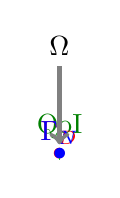
\begin{tikzpicture}[x=0.2\colwidth]
\draw (0,0) -- (1,0);
\draw[color=green, line width=4pt,-] (2/5,0) to node[anchor=south, color=green!50!black] {QoI} (4/5,0);
\node[color=red] at (0,0) {$\bullet$};
\node[color=blue] at (1,0) {$\bullet$};
\node[anchor=south,color=red] at (0,0) {$ \Gamma_D$};
\node[anchor=south, color=blue] at (1,0) {$\Gamma_N$};
\node[pin={[pin distance=1cm,pin edge={<-,solid,ultra thick}] 90:${\Omega}$}] at (0.3,0) {};
%\node[anchor=north east] at (0,0) {$0$};
%\node[anchor=north west] at (1,0) {$1$};

\end{tikzpicture}
\end{center}
\vspace{2cm}
}
%\begin{figure}
%\hspace{0.5cm}
%\subcolumn{0.333}
\innerblock{2D}{
$$g\equiv 0;\quad   h\equiv (2\pi k)\cdot \vec{n}.$$
\begin{center}
%\hspace{0.5cm}
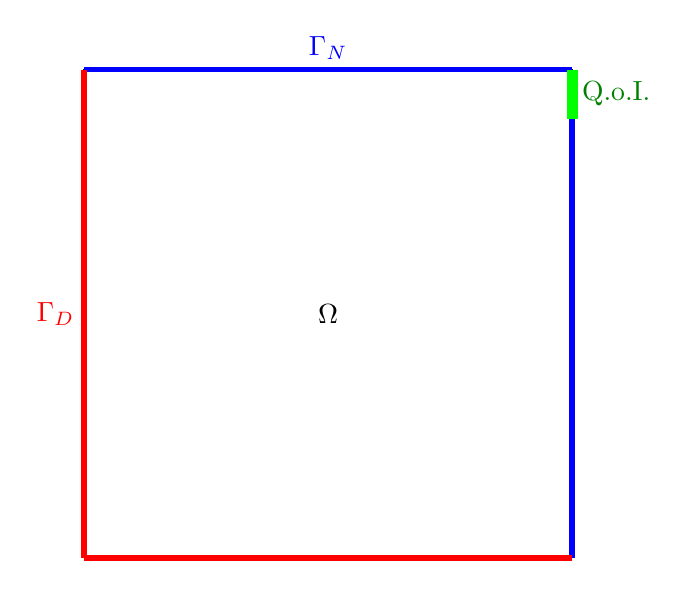
\begin{tikzpicture}[scale=6.2]

%\draw[step=0.2,gray] (0,0) grid (1,1);
%\node[anchor=east] at (0,0.2) {\tiny $\left(0,\nicefrac{1}{5}\right)$};
%\node[anchor=north] at (0.2,0) {\tiny $\left(\nicefrac{1}{5},0\right)$};

%\draw[gray] (0,0.2)--(0.2,0);
%\draw[gray] (0,0.4)--(0.4,0);
%\draw[gray] (0,0.6)--(0.6,0);
%\draw[gray] (0,0.8)--(0.8,0);
%\draw[gray] (0,1)--(1,0);
%\draw[gray] (0.2,1)--(1,0.2);
%\draw[gray] (0.4,1)--(1,0.4); 
%\draw[gray] (0.6,1)--(1,0.6);
%\draw[gray] (0.8,1)--(1,0.8);

%\node[anchor=north east] at (0,0) {\footnotesize  $(0,0)$};
%\node[anchor=south west] at (1,1) {\footnotesize $(1,1)$};


\draw[color=black] (0,0) rectangle (1,1);
\node at (0.5,0.5) {$\Omega$};

\draw[color=blue,line width=2pt](1,0) -- (1,1);
\draw[color=blue,line width=2pt](0,1) -- (1,1);


\draw[color=red,line width=2pt](0,0) -- (1,0);
\draw[color=red,line width=2pt](0,0) -- (0,1);

\node[anchor=east, color=red] at (0,1/2) {$\Gamma_D$};
\node[anchor=south, color=blue] at (1/2,1) {$\Gamma_N$};
\draw[color=green!,line width=4pt] (1,0.9) -- (1,1);
\node[anchor=west,color=green!50!black] at (1,0.95) {Q.o.I.};
\end{tikzpicture}
%}
\end{center}
%}

}
%\subcolumn{0.333}
\innerblock{3D}{
$$g\equiv 0 ;\quad   h\equiv (2\pi k)\cdot \vec{n}.$$
%\caption{Uniform triangulation of the domain $\Omega$ with discretisation step at $0.2$}
%\end{figure}


\begin{center}
%\hspace{0.5cm}
\tdplotsetmaincoords{60}{125}
\begin{tikzpicture}%[x=0.3\colwidth]
	[tdplot_main_coords,
		grid/.style={very thin,gray},
		axis/.style={->,black,thin},
		cube/.style={ very thick},
		cube hidden/.style={very thick,dashed},
		QoI/.style={very thick,fill=green},%,pattern=custom north west lines, hatchcolor=green!100!black,opacity=1},
		%x=-2cm,
		%y=2cm,
		%z=2cm,
		scale=3.4
		]
	%draw a grid in the x-y plane
%	\foreach \x in {-0.5,0,...,2.5}
%		\foreach \y in {-0.5,0,...,2.5}
%		{
%			\draw[grid] (\x,-0.5) -- (\x,2.5);
%			\draw[grid] (-0.5,\y) -- (2.5,\y);
%		}			

	%draw the axes
	\draw[axis] (1,0,0) -- (1.5,0,0) node[anchor=west]{$x$};
	\draw[axis] (0,1,0) -- (0,1.5,0) node[anchor=west]{$y$};
	\draw[axis] (0,0,1) -- (0,0,1.5) node[anchor=west]{$z$};

	%draw the bottom of the cube
	\draw[cube,dashed, opacity=1] (0,0,0) -- (0,1,0) -- (1,1,0) -- (1,0,0) -- cycle;
	
	%draw the back-right of the cube
	\draw[cube,dashed,opacity=1] (0,0,0) -- (0,1,0) -- (0,1,1) -- (0,0,1) -- cycle;

	%draw the back-left of the cube
	\draw[cube,dashed,opacity=1] (0,0,0) -- (1,0,0) -- (1,0,1) -- (0,0,1) -- cycle;

	\node[pin={[pin distance=1cm,pin edge={<-,red,ultra thick,dashed}] 70:$\color{red}{\Gamma_D}$}] at (0,0.5,0.8) {};
	\node at (0.7,0.6,0.5){$\Omega$};
	%draw the front-right of the cube
	\draw[cube,fill=blue ,opacity=0.5] (1,0,0) -- (1,1,0) -- (1,1,1) -- (1,0,1) -- cycle;

	%draw the front-left of the cube
	\draw[cube,fill=blue,opacity=0.5] (0,1,0) -- (1,1,0) -- (1,1,1) -- (0,1,1) -- cycle;

	%draw the top of the cube
	\draw[cube,fill=blue,opacity=0.5] (0,0,1) -- (0,1,1) -- (1,1,1) -- (1,0,1) -- cycle;
	\draw[cube] (0,0,1) -- (0,1,1) -- (1,1,1) -- (1,0,1) -- cycle;
	
	\node[pin={[pin distance=1cm,pin edge={<-,solid,blue,ultra thick}] 110:$\color{blue}{\Gamma_N}$}] at  (1/2,0.05,1) {};
	
	%draw the QoI
	\draw[QoI] (0.9,0.9,1) -- (0.9,1,1) -- (1,1,1) -- (1,0.9,1) -- cycle;
%	%draw the QoI
	\draw[QoI] (1,0.9,0.9) -- (1,0.9,1) -- (1,1,1) -- (1,1,0.9) -- cycle;
%	%draw the QoI
	\draw[QoI] (0.9,1,0.9) -- (0.9,1,1) -- (1,1,1) -- (1,1,0.9) -- cycle;
	
	\node[pin={[pin distance=1.7cm,pin edge={<-,solid,green,ultra thick}] 0:$\color{green!50!black}{QoI}$}] at  (1,1,1) {};
	
	%\node[anchor=south, color=blue] at (0,1/2,1) {$\Gamma_N$};
	%\node[anchor=south, color=red] at (1/2,0,1) {$\Gamma_D$};
	%\node[anchor=west, color=green!50!black] at (0,1,1/2) {$QoI$};
	
\end{tikzpicture}
%}
\end{center}
%\vspace{.5cm}
}
%\end{subcolumns}
\end{multicols}




}%



\end{columns}



\begin{columns}
%%%%%%%%%%%%
%%
  %%
 \column{0.3333} 
 %%
 %%
 %%%%%%%%%%%%

% \block{1D numerical results}{%
% 
%\newlength{\plotwidth}
%\newlength{\plotheight}
%
%\setlength{\plotheight}{15cm}
%    \setlength{\plotwidth}{20cm}
%
% \begin{tikzfigure}[Uniform {$p$-refinements} for $k\simeq 20$ wavelengths, $h(2k\pi)\gg 1$.]
%%  \begin{center}
%   % \ref{legend_precise}
%   
%    
%   % \setlength{\plotheight}{5.9cm}
%%\ref{legend_2D_bounds}\\
%%\tikzstyle{every node}=[font=\footnotesize]
%%   \vspace{-0.2cm}
%%\hspace{-0.9cm}
%\begin{tikzpicture}
%\begin{axis}[width=\plotwidth,height=\plotheight,
%%scale only axis,
%%xmode=log,
%%xmin=2.50345664582937,
%%xmax=157.128720064702,
%xtick={3,5,10,15},
%xticklabels={3,{5},{10},{15}},
%xminorticks=true,
%ytick={10e{-3},10e{-1},10e{2},10e{4}},
%yticklabels={$10^{-3}$,$10^{-1}$,$10^{2}$,$10^{4}$},
%xlabel={D.o.f.s per wavelength},
%ymode=log,
%%ymin=0.000494125487062414,
%%ymax=10000,%204.11905803267,
%yminorticks=true,
%ylabel={Relative error in \%},
%%legend style={ draw=black,fill=white,legend cell align=left},
%%legend to name=legend_precise
%%legend pos= north east,
%]
%%\legend{$\abs{l(e_h)}$,Classical bound,New bound}
%{\addplot [color=red,solid,line width=4pt]
%  table[row sep=crcr]{
%3.23976742401447	526.272764541084	\\
%6.43044746281661	508.156101113134	\\
%9.62112750161874	4.93030129193148	\\
%12.8118075404209	0.0743677510892578	\\
%16.002487579223	0.000742580239625024	\\
%%19.1931676180251	5.09804147768799e-06	\\
%}
%node[pin={[pin edge={<-,solid,red,ultra thick}]-90:$\abs{l(e_h^*)}$}] at (4.23976742401447,526.272764541084) {};
%%\addlegendentry{$\abs{l(e_h)}$}
%}
%{\addplot [color=black!50!green,dotted,mark=triangle,mark options={solid,,rotate=180},line width=4pt]
%  table[row sep=crcr]{
%  3.23976742401447	17545.310906375	\\
%6.43044746281661	83790.7436006804	\\
%9.62112750161874	10.6410983067026	\\
%12.8118075404209	0.104026565549748	\\
%16.002487579223	0.00104313592634005	\\
%%19.1931676180251	7.07065405758037e-06	\\
%}
%node[pin={[pin edge={<-,solid,black!50!green,ultra thick}] 0:Classical estimate}] at (6.43044746281661,83790.7436006804) {};
%}
%{\addplot [color=blue,dashed,mark=+,line width=4pt,mark options={solid}]
%  table[row sep=crcr]{
%3.23976742401447	2021.58595776932	\\
%6.43044746281661	511.005884240018	\\
%9.62112750161874	6.68626165611229	\\
%12.8118075404209	0.102706477792951	\\
%16.002487579223	0.0010432712465022	\\
%%19.1931676180251	7.07064812859771e-06	\\
%}
%node[pin={[pin edge={<-,solid,blue,ultra thick}] -90:New estimate}] at (9.62112750161874,6.68626165611229) {};
%%\addlegendentry{New bounds}
%}
%
%\end{axis}
%\end{tikzpicture}
%%\end{center}
%%\caption{}
%\end{tikzfigure}
%}%


%\note[targetoffsetx=-3cm, targetoffsety=-2cm, angle=0, radius=0cm,width=7cm, rotate=10, connection, linewidth=.2cm,
%     roundedcorners=30, innersep=1cm]{\centering\vspace{1.5cm}\textbf{Published!}
%%\scriptsize
%%V.~Darrigrand, D.~Pardo, and I.~Muga.\\
%% Goal-oriented adaptivity using unconventional error representations for the 1d Helmholtz equation.\\
%% {\em Computers \& Mathematics with Applications}, 2015.%
% }
%%%%%%%%%%%%%
%%%
%  %%
% \column{0.3333} 
% %%
% %%
% %%%%%%%%%%%%
% 
%\block{2D numerical results}{%
%
%
% \begin{tikzfigure}[Uniform $p$-refinements, for $k=30$ wavelengths, $h(2k\pi)\gg 1$.]
%%  \begin{center}
%   % \ref{legend_precise}
%   
%    \setlength{\plotheight}{15cm}
%    \setlength{\plotwidth}{20cm}
%   % \setlength{\plotheight}{5.9cm}
%%\ref{legend_2D_bounds}\\
%%\tikzstyle{every node}=[font=\footnotesize]
%%   \vspace{-0.2cm}
%%\hspace{-0.9cm}
%\begin{tikzpicture}
%\begin{axis}[%
%width=\plotwidth,height=\plotheight,
%%xmode=log,
%xmin=1.5,
%xmax=9,
%xlabel={D.o.f.s per wavelength},
%xtick={2,3,4,6,8},
%xticklabels={2,3,4,6,8},
%ytick={10e{-3},10e{-1},10e{1},10e{3},10e{6}},
%yticklabels={$10^{-3}$,$10^{-1}$,$10^{1}$,$10^{3}$,$10^{6}$},
%%xticklabels={},
%ymode=log,
%ylabel={Relative error in \%},
%%legend pos= outer north east,
%%legend style={draw=black,fill=white,legend cell align=left},
%]
%\addplot [color=red,solid,line width=4pt,]
%  table[x=DOF,y=LE]{bounds_2D.txt}
%  node[pin={[pin edge={<-,solid,red,ultra thick}]-90:$\abs{l(e_h^*)}$}] at (2.3805928707368218,132.15818485126883) {};
%%node[pin={[pin distance=1cm,pin edge={<-,solid,red,thick}] -90:$\abs{l(e_h)}$}] at (2.5927248644,145.5102634148) {};
%%\addlegendentry{$l(e_h)$};
%
%\addplot [color=black!50!green,dotted,mark=triangle,mark options={solid,rotate=180},line width=2pt,]
%  table[x=DOF,y=Classical]{bounds_2D.txt}
%  node[pin={[pin edge={<-,solid,black!50!green,ultra thick}] 0:Classical estimate}] at (4.7376155150307051 ,  16098132.017135398) {};
%%node[pin={[pin edge={<-,solid,black!50!green,thick}] 0:Classical bound}] at (4.9497474683,3478.7271859448) {};
%%\addlegendentry{Classical bound};
%
%\addplot [color=blue,dashed,mark=+,mark options={solid},line width=4pt,]
%  table[x=DOF,y=Alternative]{bounds_2D.txt}
%  node[pin={[pin edge={<-,solid,blue,ultra thick}] -90:New estimate}] at (5.9161268371776465   ,  4.3979422214161294 ) {};
%%node[pin={[pin distance=1cm,pin edge={<-,solid,blue,thick}] -90:$\tilde{b}=\scalaire{\grad \cdot}{\grad \cdot}_{L^2}$}] at (3.7712361663, 1191.3435988333) {};
%%\addlegendentry{$\tilde{b}=\scalaire{\grad \cdot}{\grad \cdot}_{L^2}$};
%\end{axis}
%
%\end{tikzpicture}
%%\end{center}
%%\caption{}
%\end{tikzfigure}
%}%
%%%%%%%%%%%%%
%%%
%  %%
% \column{0.3333} 
% %%
% %%
% %%%%%%%%%%%%
%
%\block{3D numerical results}{%
%
% \begin{tikzfigure}[Uniform $p$-refinements, for $k=3$ wavelengths, $h(2k\pi)\gg 1$.]
%%  \begin{center}
%   % \ref{legend_precise}
%   
%    \setlength{\plotheight}{15cm}
%    \setlength{\plotwidth}{20cm}
%   % \setlength{\plotheight}{5.9cm}
%%\ref{legend_2D_bounds}\\
%%\tikzstyle{every node}=[font=\footnotesize]
%%   \vspace{-0.2cm}
%%\hspace{-0.9cm}
%\begin{tikzpicture}
%\begin{axis}[%
%width=\plotwidth,height=\plotheight,
%%xmode=log,
%xmin=1.5,
%xmax=9,
%xlabel={D.o.f.s per wavelength},
%xtick={2,3,4,6,8},
%xticklabels={2,3,4,6,8},
%ytick={10e{-3},10e{-1},10e{1},10e{3},10e{4}},
%yticklabels={$10^{-3}$,$10^{-1}$,$10^{1}$,$10^{3}$,$10^{4}$},
%%xticklabels={},
%ymode=log,
%ylabel={Relative error in \%},
%%legend pos= outer north east,
%%legend style={draw=black,fill=white,legend cell align=left},
%]
%\addplot [color=red,solid,line width=4pt,]
%  table[x=DOF,y=LE]{bounds_3D.txt}
%  node[pin={[pin edge={<-,solid,red,ultra thick}]-90:$\abs{l(e_h^*)}$}] at (2.6261511956655523 ,100.71786639514887) {};
%%node[pin={[pin distance=1cm,pin edge={<-,solid,red,thick}] -90:$\abs{l(e_h)}$}] at (2.5927248644,145.5102634148) {};
%%\addlegendentry{$l(e_h)$};
%
%\addplot [color=black!50!green,dotted,mark=triangle,mark options={solid,rotate=180},line width=4pt,]
%  table[x=DOF,y=Classical]{bounds_3D.txt}
%  node[pin={[pin edge={<-,solid,black!50!green,ultra thick}] 0:Classical estimate}] at (3.8387107053617489 ,  3434.4857095762368) {};
%%node[pin={[pin edge={<-,solid,black!50!green,thick}] 0:Classical bound}] at (4.9497474683,3478.7271859448) {};
%%\addlegendentry{Classical bound};
%
%\addplot [color=blue,dashed,mark=+,mark options={solid},line width=4pt,]
%  table[x=DOF,y=Alternative]{bounds_3D.txt}
%  node[pin={[pin edge={<-,solid,blue,ultra thick}] -90:New estimate}] at (5.0511740428693495   , 12.581899208609796 ) {};
%%node[pin={[pin distance=1cm,pin edge={<-,solid,blue,thick}] -90:$\tilde{b}=\scalaire{\grad \cdot}{\grad \cdot}_{L^2}$}] at (3.7712361663, 1191.3435988333) {};
%%\addlegendentry{$\tilde{b}=\scalaire{\grad \cdot}{\grad \cdot}_{L^2}$};
%\end{axis}
%\end{tikzpicture}
%%\end{center}
%%\caption{}
%\end{tikzfigure}
%}%
%
%%%%%%%%%%%%%
%
%
%
%
% \end{columns} 
%
%\begin{columns}
%
%\column{0.25}
%\block{Formations}{
%\begin{itemize}
%\item Teaching (192h eq. TD in 2014-2015);
%\item Various formations on scientific computing (python, fortran, MPI);
%\item Languages certifications (DELE-C1 and CAE).
%\end{itemize}
%
%}
%\column{0.5}
%
%\block{Work in progress and future work}{
%\begin{itemize}
%\item Multi-D Goal-oriented Adaptivity;
%\item Theoretical proof of if there exists a $\hat{b}$ such that the alternative estimate is sharper than the classical one;
%\item Widen the study to other kind of problems (eg. diffusion-convection problems);
%\item Application to non-linear quantities of interest.
%\end{itemize}
%%
%}
%\column{0.25}
%
%
%\block{Mobility}{
%\begin{itemize}
%\item Bilbao (18 months);
%\item Pau (12 months);
%\item Valparaiso (6 months).
%\end{itemize}
%%
%}
%
%\block{}{
%\begin{center}
%\begin{tikzpicture}
%\begin{scope}[it_style/.style={rectangle, fill=mygray!20,line width=4pt,}]
%
%\node(phantom){};
%\shade[ball color=mygreen!30] (phantom) ellipse [x radius=30cm, y radius=8cm];
%\node[left=of phantom](WIP){};
%\node[left=15 of WIP](phantom_wip){};
%\node[above=of phantom_wip](MDGOA){};
%\node[above=of MDGOA](PROOF){};
%\node[below=of phantom_wip](Probs){};
%\node[below=of Probs](NLQOI){};
%
%\draw (MDGOA) node [it_style] {Multi-D Goal-oriented Adaptivity};
%\path (PROOF) node [it_style] {Theoretical proof};
%\path (Probs) node [it_style] {Widen the range of problems};
%\path (NLQOI) node [it_style] {Application to non-linear QoI};
%
%\node[right=15 of phantom](Mob){};
%\node[above=of Mob](BIO){};
%\node[below=of Mob](VALPO){};
%
%\path (Mob) node [it_style] {Pau (12 monthes)};
%\path (BIO) node [it_style] {Bilbao (18 monthes)};
%\path (VALPO) node [it_style] {Valparaiso (6 monthes)};
%
%\end{scope}
% \begin{scope}[mindmap,
%every node/.style={concept, circular drop shadow,execute at begin node=\hskip0pt, scale=1},
%%root concept/.style={concept color=mygreen!50,faded/.style={concept color=mygreen!50}},
%level 1 concept/.append style={level distance=0.1\textwidth},
%level 2 concept/.append style={level distance=0.07\textwidth},
%WIP/.style={concept color=mybrown!50},
% ]
% \node[root concept]{}% root
% child[grow=180,WIP]{node{Work in Progress} 
% [clockwise from=-90]
%  child{node{Multi-D Goal-oriented Adaptivity}}
%     child { node{Theoretical proof}}
%    child{node{Application to non-linear QoI}}
%    child{node[ellipse]{Widen the range of problems}}
%    }
%child[grow=0,WIP]{node{Mobility} 
% [clockwise from=60]
%  child{node{Bilbao (18 monthes) }}
%     child{node{Pau (12 monthes)}}
%    child{node{Valparaiso (6 monthes)}}
%    };
%  \end{scope}
%\end{tikzpicture}
%\end{center}
%
%}

%\begin{columns}
%%%
%  %%
% \column{0.5} 
% %%
% %%
% 
% \block{Work in progress}{
% \begin{itemize}
%\item Application to multi-D goal oriented adaptive procedure
%\item 
%\end{itemize}
%}
%%%%%%%%%%%%%
%%%
%  %%
% \column{0.5} 
% %%
% %%
% %%%%%%%%%%%%
% 
%\block{Formations and Mobility}{blabla}
%%%%%%%%%%%%%
%
 \end{columns} 
  \end{document}